% geoweb.tex
\documentclass{beamer}
%\usetheme{roadkill}
%\usecolortheme[]{albatross}
\setbeamertemplate{navigation symbols}{} 
\usebackgroundtemplate{
	
\includegraphics[width=\paperwidth,
	height=\paperheight]{backdrop.png}
}
%\setbeamertemplate{itemize items}{\includegraphics[width=10px]{reflector.jpg}}

%\definecolor{safetyorange}{RGB}{232, 118, 0}
\setbeamercolor{background canvas}{bg=white}
\setbeamercolor{frametitle}{fg=black}
%\setbeamercolor{block title}{fg=white}
%\setbeamercolor{block body}{fg=white}
%\setbeamerfont{frametitle}{parent=structure,size=\huge}

\usepackage{graphicx}
\usepackage{datatool}
\usepackage{listings}
\usepackage{caption}
\usepackage{changepage}

\usepackage{hyperref}
\hypersetup{colorlinks=true, linkcolor=blue, citecolor=blue, urlcolor=blue}


%Footnote like stuff
\usepackage[absolute,overlay]{textpos} 
\newenvironment{reference}[2]{% 
  \begin{textblock*}{\textwidth}(#1,#2) 
      \footnotesize\it\bgroup\color{black}}{\egroup\end{textblock*}} 

% items enclosed in square brackets are optional; explanation below
\title[PDFTitle]{Barriers to FOSS4G Adoption}
\subtitle[Sub]{OSGeo-Live case study}
\author[A. Mandel]{Alex Mandel, PhD} %\\
	%\footnotesize Co-Author: Paul Haverkamp}
\institute[UCD]{
  Geography Graduate Group\\
  University of California, Davis\\
  %Davis, California 95616\\[1ex]
  \texttt{aimandel@ucdavis.edu}\\
  @aimandel
}
\date[Sep 2014]{September 10, 2014}



\begin{document}
\section{Intro}
\begin{frame}[plain]
  \titlepage
   \begin{reference}{35mm}{85mm}
		\tiny \href{http://creativecommons.org/licenses/by-nc-sa/3.0/}{Creative Commons Attribution Share-alike Non-commercial}
		
\includegraphics[width=22px]{cc-a-nc-sa-88x31.png}
   \end{reference} 
  %\footnote{Creative Commons Attribution Share-alike Non-commercial}
\end{frame}

%\begin{frame}{Citizen Science aka Crowdsourcing}
%    \vspace{-1in}
%	\begin{itemize}
%		\item I
%			\begin{itemize}
%				\item A
%				\item B
%				\item C
%			\end{itemize}		
%		\item II
%			\begin{itemize}
%				\item A
%				\item B
%				\item C
%			\end{itemize} 
%	\end{itemize}
%\end{frame}

\section{Downloads}


\begin{frame}{Downloads}
\vspace{-.25in}
	\begin{minipage}{\textwidth}
		\begin{center}
			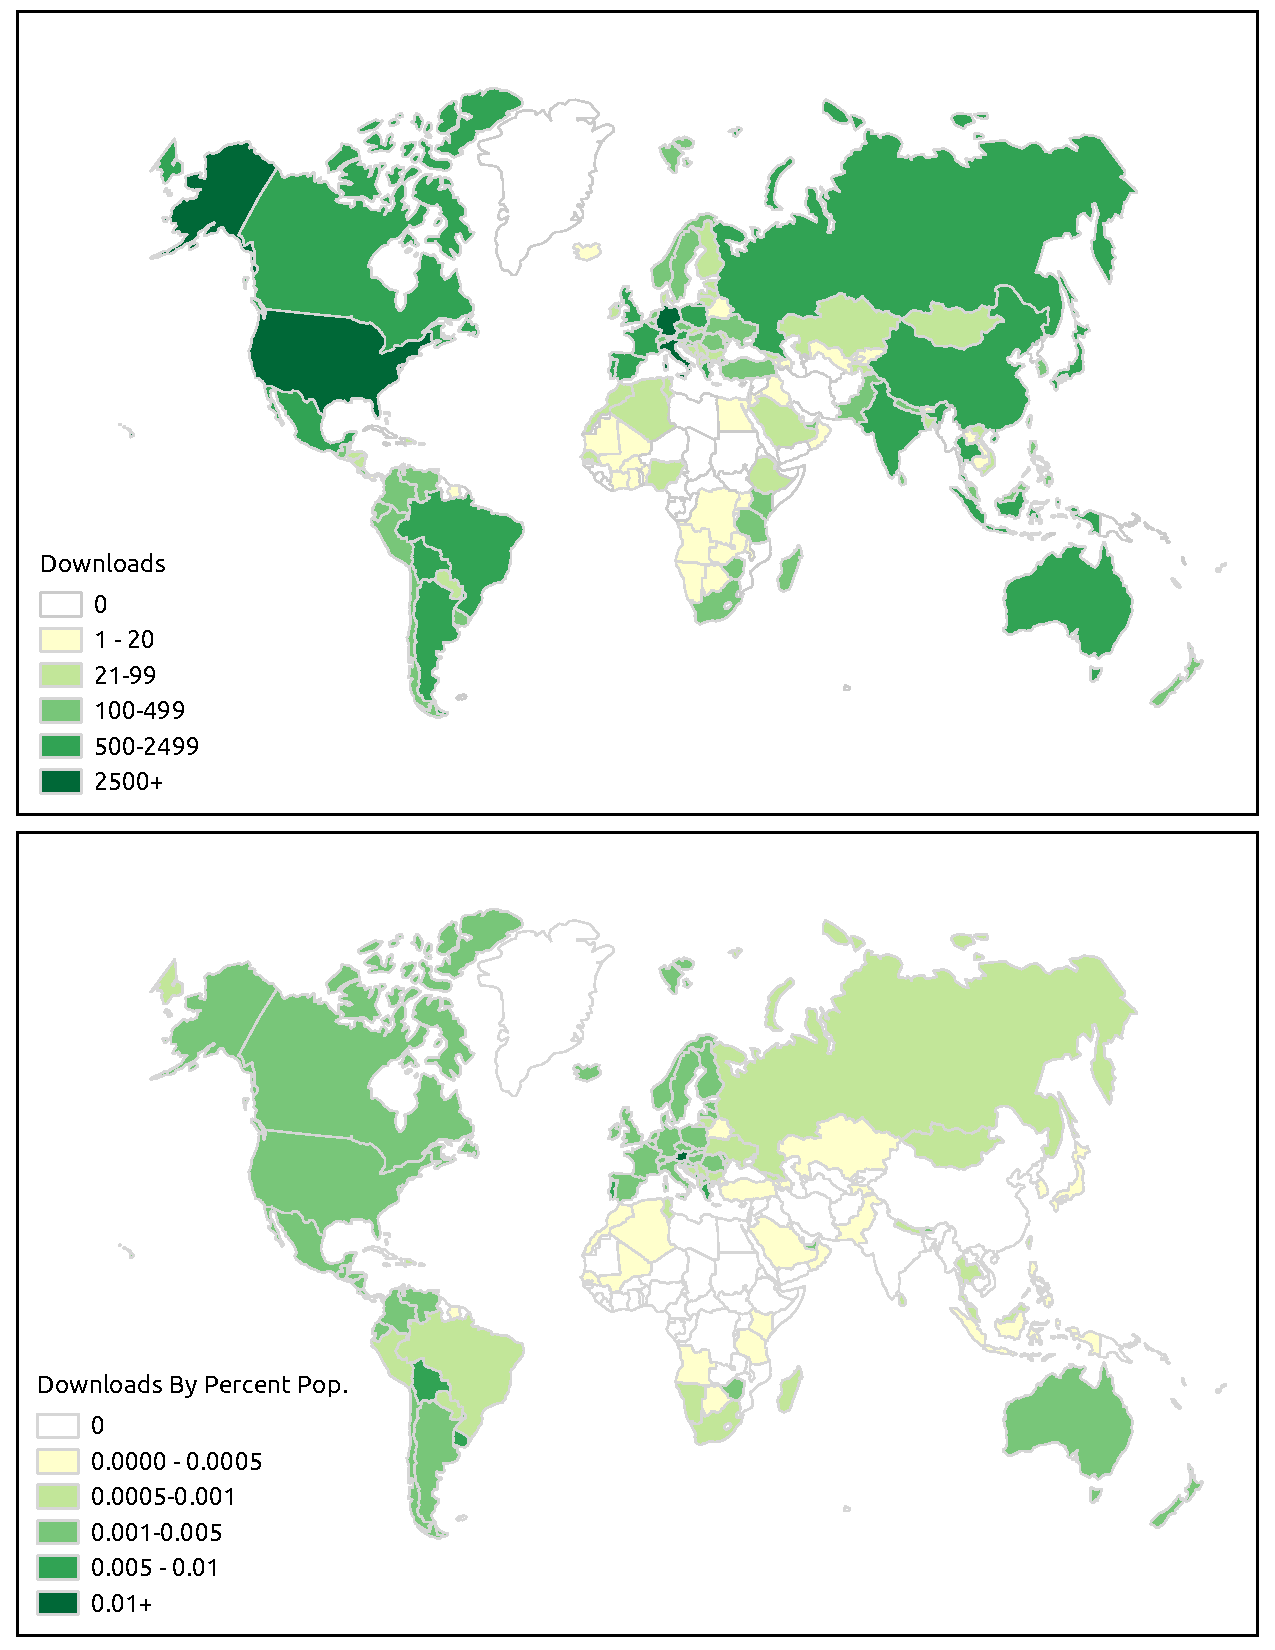
\includegraphics[width=.6\textwidth]{DownloadMapQGIS.pdf}
		\end{center}
	\end{minipage}
	%\footnote{\tiny{Projection: Van der Grinten I}}
\end{frame}

\DTLloadrawdb{top10down}{top10downloads.csv}
\DTLloadrawdb{top10downbypop}{top10downbypop.csv}

\begin{frame}{OSGeo-Live Downloads: Top 10 Countries \\ \tiny{(Versions 6.0 \& 6.5)}}
\vspace{-.5in}
%\begin{adjustwidth}{-2em}{0em}
	%\begin{minipage}{\textwidth}
	\begin{scriptsize}
	\begin{columns}[T]
	\begin{column}{0.3\textwidth}
		
		\begin{table}
		%\centering
		\caption{\scriptsize{Total Downloads}}
	%\caption{}
	%\begin{subtable}
		\begin{tabular}{l}
			\DTLdisplaydb{top10down}		
		\end{tabular}
	%\end{subtable}
	%\qquad
		\end{table}
	\end{column}
	\begin{column}{0.001\textwidth}
	\end{column}
	\begin{column}{0.62\textwidth}
		
		\begin{table}
		%\centering
		\caption{\scriptsize{Downloads by Percent Population}}
	%\begin{subtable}{1\linewidth}\centering
		\begin{tabular}{l}
	%		\centering
			\DTLdisplaydb{top10downbypop}
		\end{tabular}
		
	%\end{subtable}
		
		\label{table:top10}
		\end{table}
	\end{column}
	\end{columns}
	\end{scriptsize}		
	%\end{minipage}	
%\end{adjustwidth}
\end{frame}

\section{Participation}
\begin{frame}{Regional Participation}
\vspace{-.3in}
	\begin{center}
		%\hspace*{1em}
		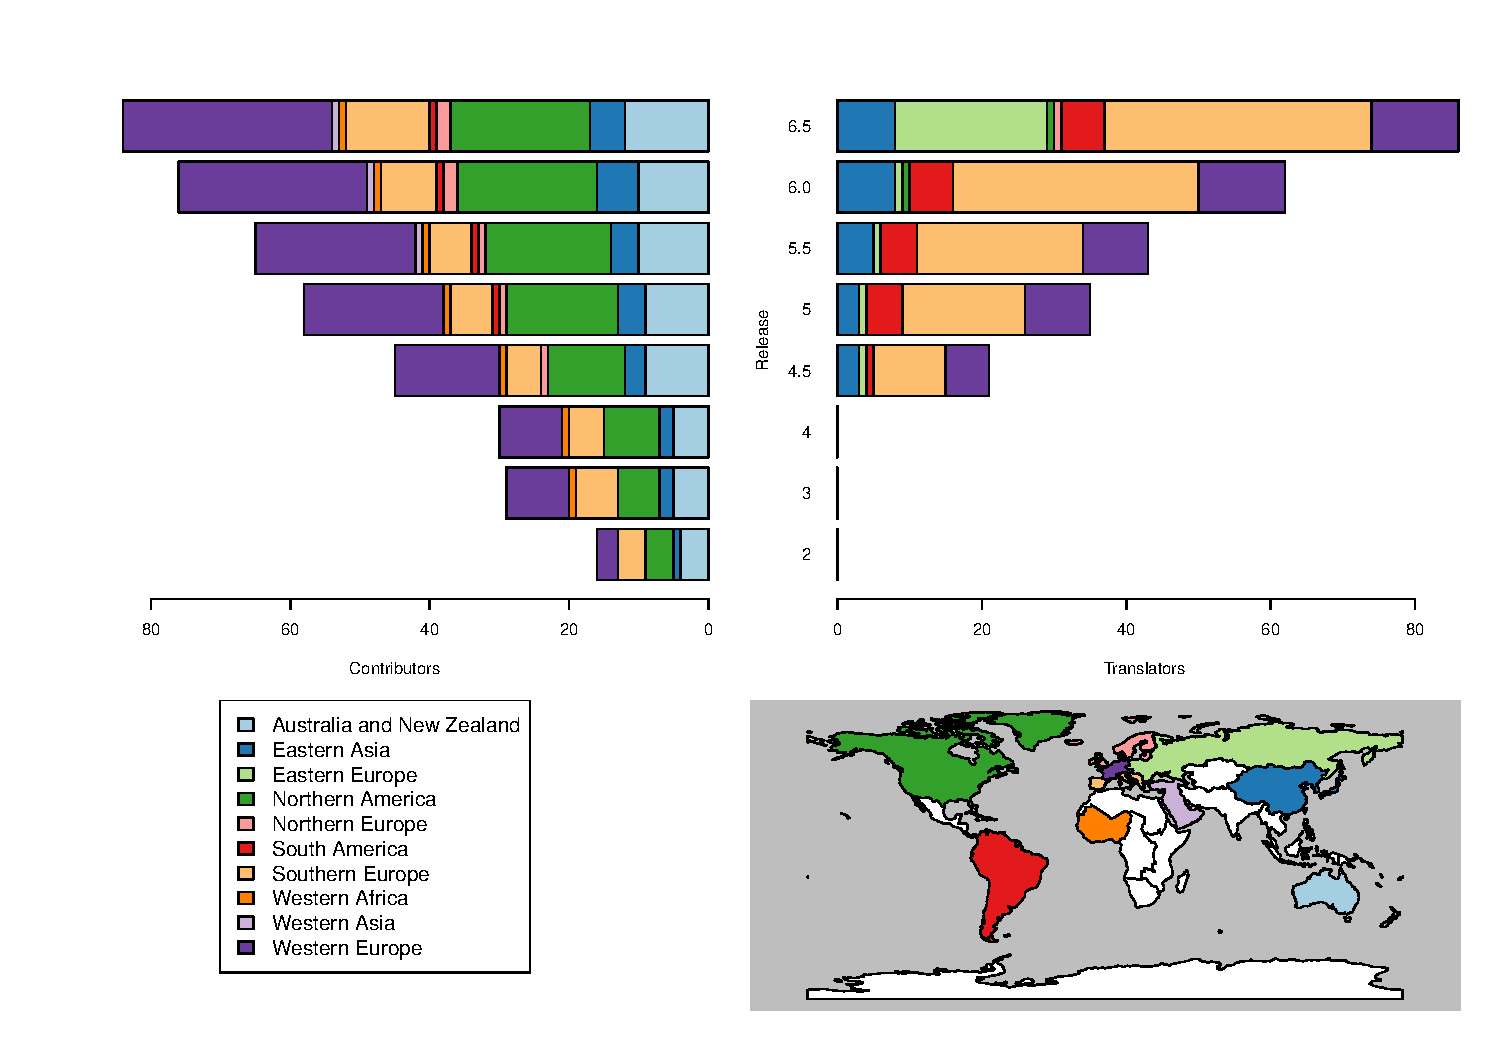
\includegraphics[width=1\textwidth]{RegionalParticipation.pdf}
		
		%\hspace*{2em}\textbf{\url{http://www.wildlifecrossing.net/california/}}
	\end{center}
\end{frame}

\begin{frame}{Important Variables}
	\begin{center}
		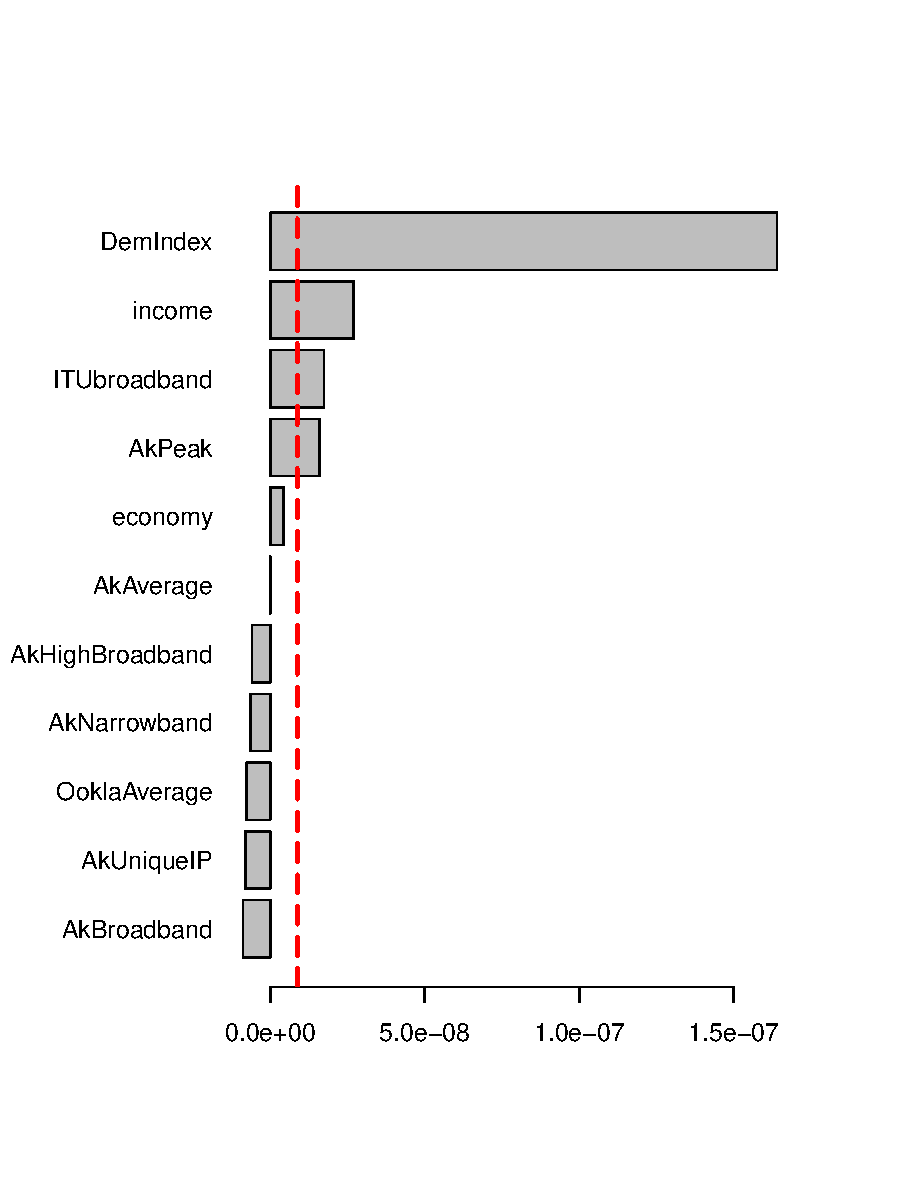
\includegraphics[width=.5\textwidth]{ImportantVariables-caret.pdf}
	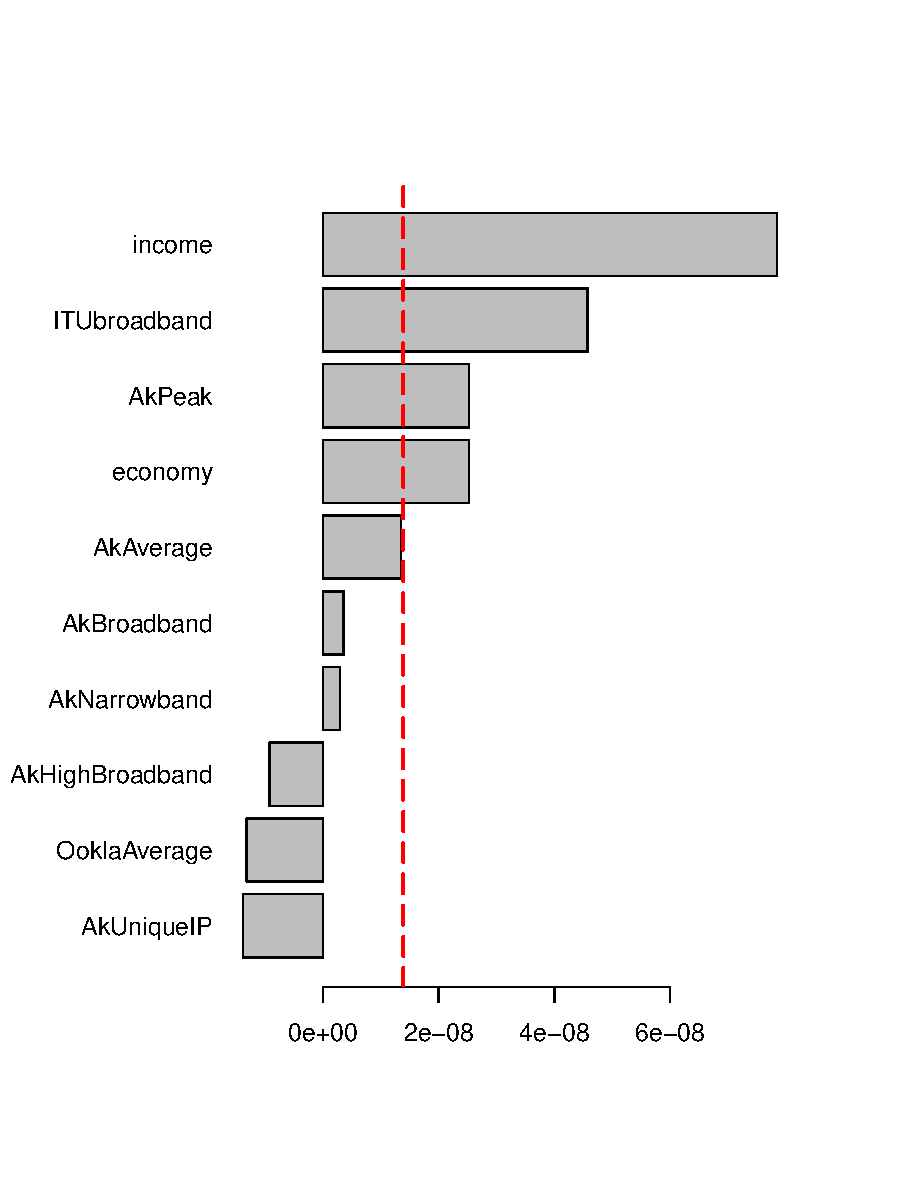
\includegraphics[width=.5\textwidth]{ImportantVariables-NoDemIndex.pdf}
	\end{center}
\end{frame}

\section{Regression}
\begin{frame}{Important Relationships}
	\begin{center}
			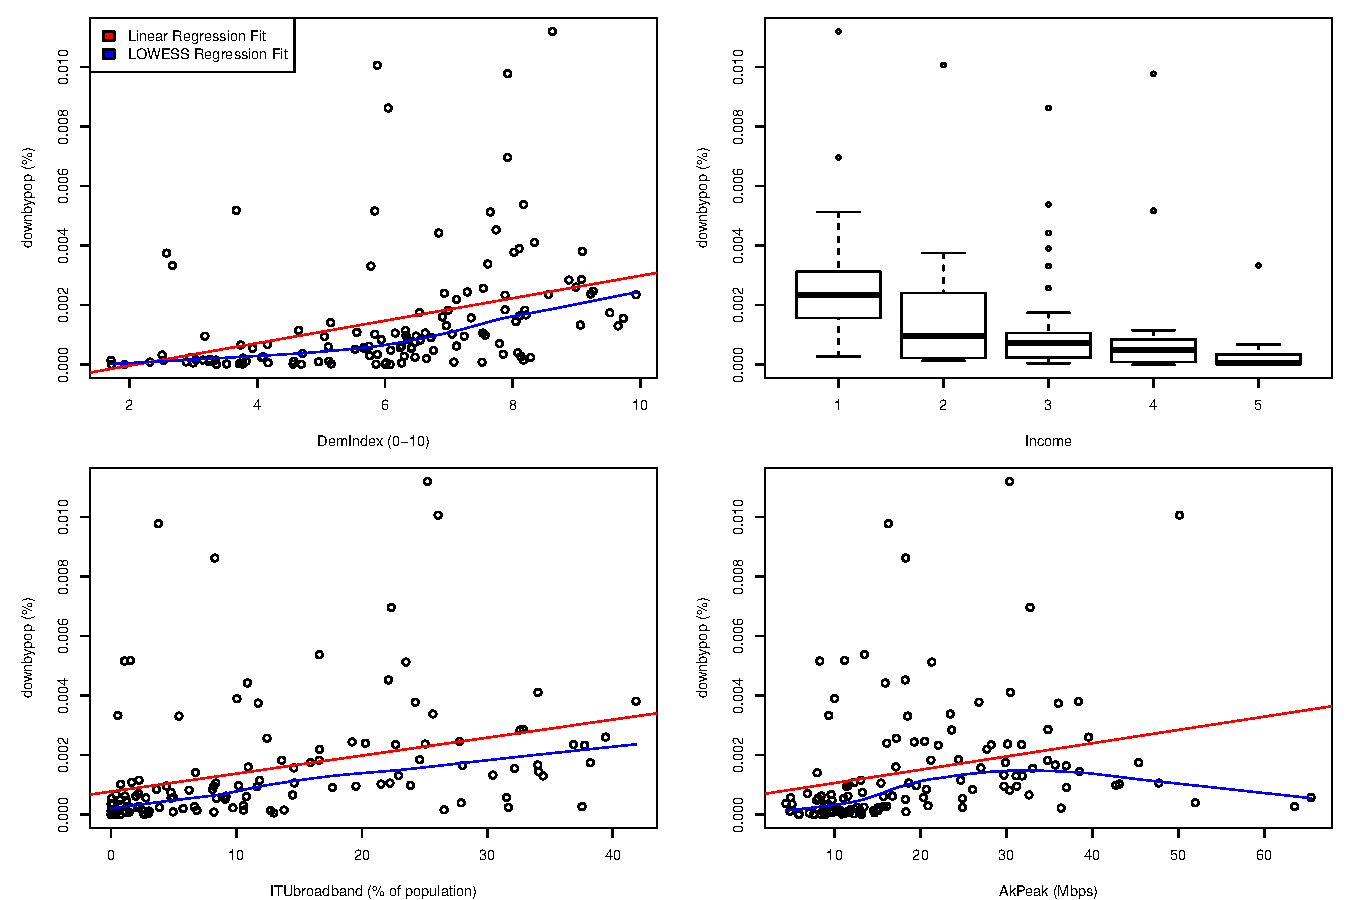
\includegraphics[width=1\textwidth]{ImportantVarGraph.pdf}	
	\end{center}
\end{frame}

\section{Credits}
\begin{frame}{Special Thanks}
	\begin{itemize}
		\item OSGeo-Live Team and Community \url{http://live.osgeo.org}
		\item Jim Quinn and the \href{http://ice.ucdavis.edu}{Information Center for the Environment}
		%\item Link Example %\begin{small}
%\url{http://www.wildlifecrossing.net/california/android}
%\end{small}
		\item Questions?
		\begin{center}
			%\includegraphics[width=0.5\textwidth]{File.png}
		\end{center}
	\end{itemize}
\end{frame}


% Columns example
%\begin{frame}{Currency of the GeoWeb}	
%		\begin{columns}[t]
%			\column{.59\textwidth} % column designated by a command
%     			\begin{block}{KML}
%      				%\tiny\lstinputlisting{world.kml}
%   				\end{block}
%    		\column{.39\textwidth}		
%				\begin{block}{GeoJson}
%					%\tiny\lstinputlisting{world.geojson}
%				\end{block}
%				\begin{itemize}
%					\item GML - not shown here
%				\end{itemize}
%		\end{columns}
%\end{frame}


\end{document}